\newproblem{21.5a}{Find the equation of the circle graphed below.

\noindent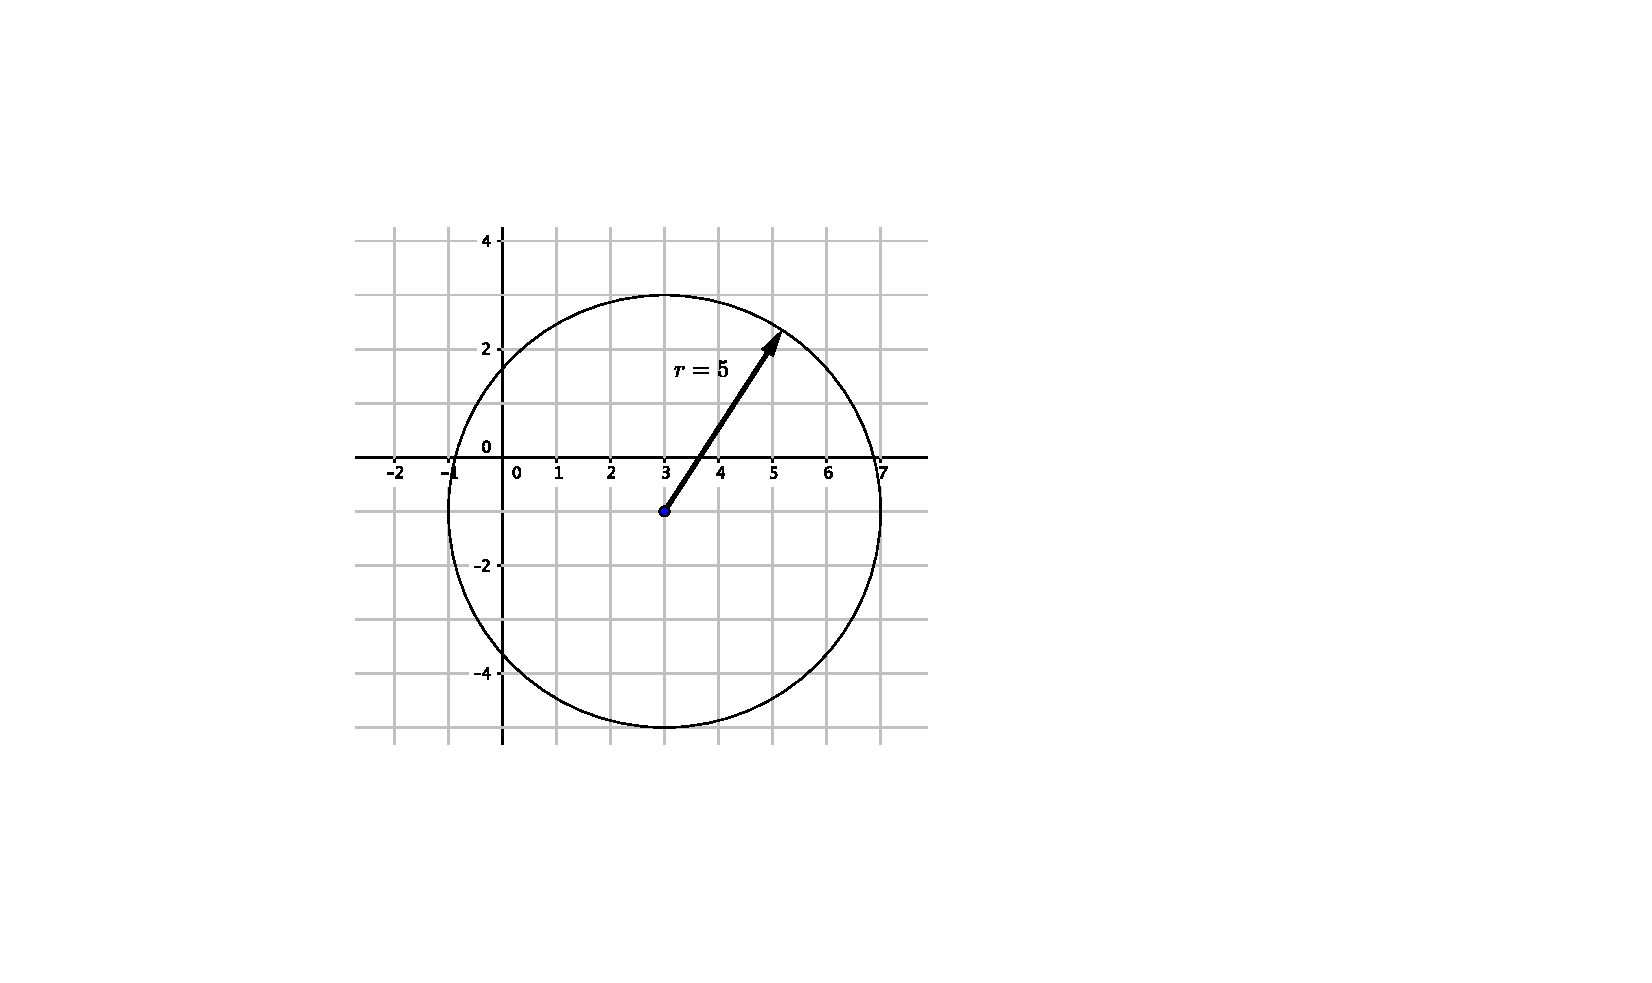
\includegraphics[height=2.5in]{MAT100_Number21a.pdf}}
{\begin{tabular}{lllll}
 &&&&\\ Correct form of the equations&&$(x-h)^2+(y-k)^2=r^2$&&Add 2 points\\
Correct center of the circle&&$(3,-1)$&&Add 2 points\\
Correct radius of the equation&&$r=5$&&Add 2 points\\ &&&&\\ \end{tabular}}




\newproblem{21.5b}{Find the equation of the circle graphed below.

\noindent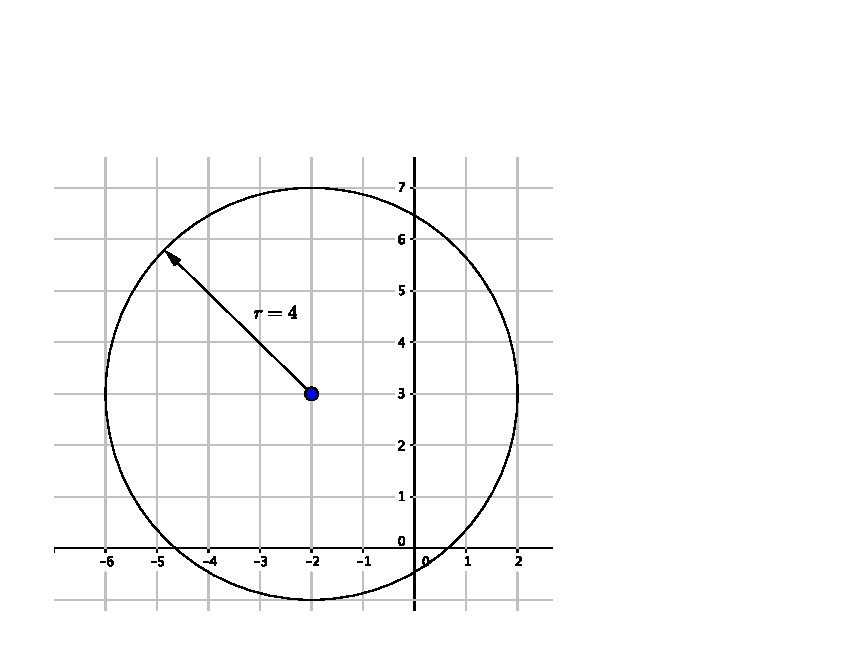
\includegraphics[height=2.5in]{MAT100_Number21b.pdf}}
{\begin{tabular}{lllll}
 &&&&\\ Correct form of the equations&&$(x-h)^2+(y-k)^2=r^2$&&Add 2 points\\
Correct center of the circle&&$(-2,3)$&&Add 2 points\\
Correct radius of the equation&&$r=4$&&Add 2 points\\ &&&&\\ \end{tabular}}

\newproblem{21.5c}{Find the equation of the circle graphed below.

\noindent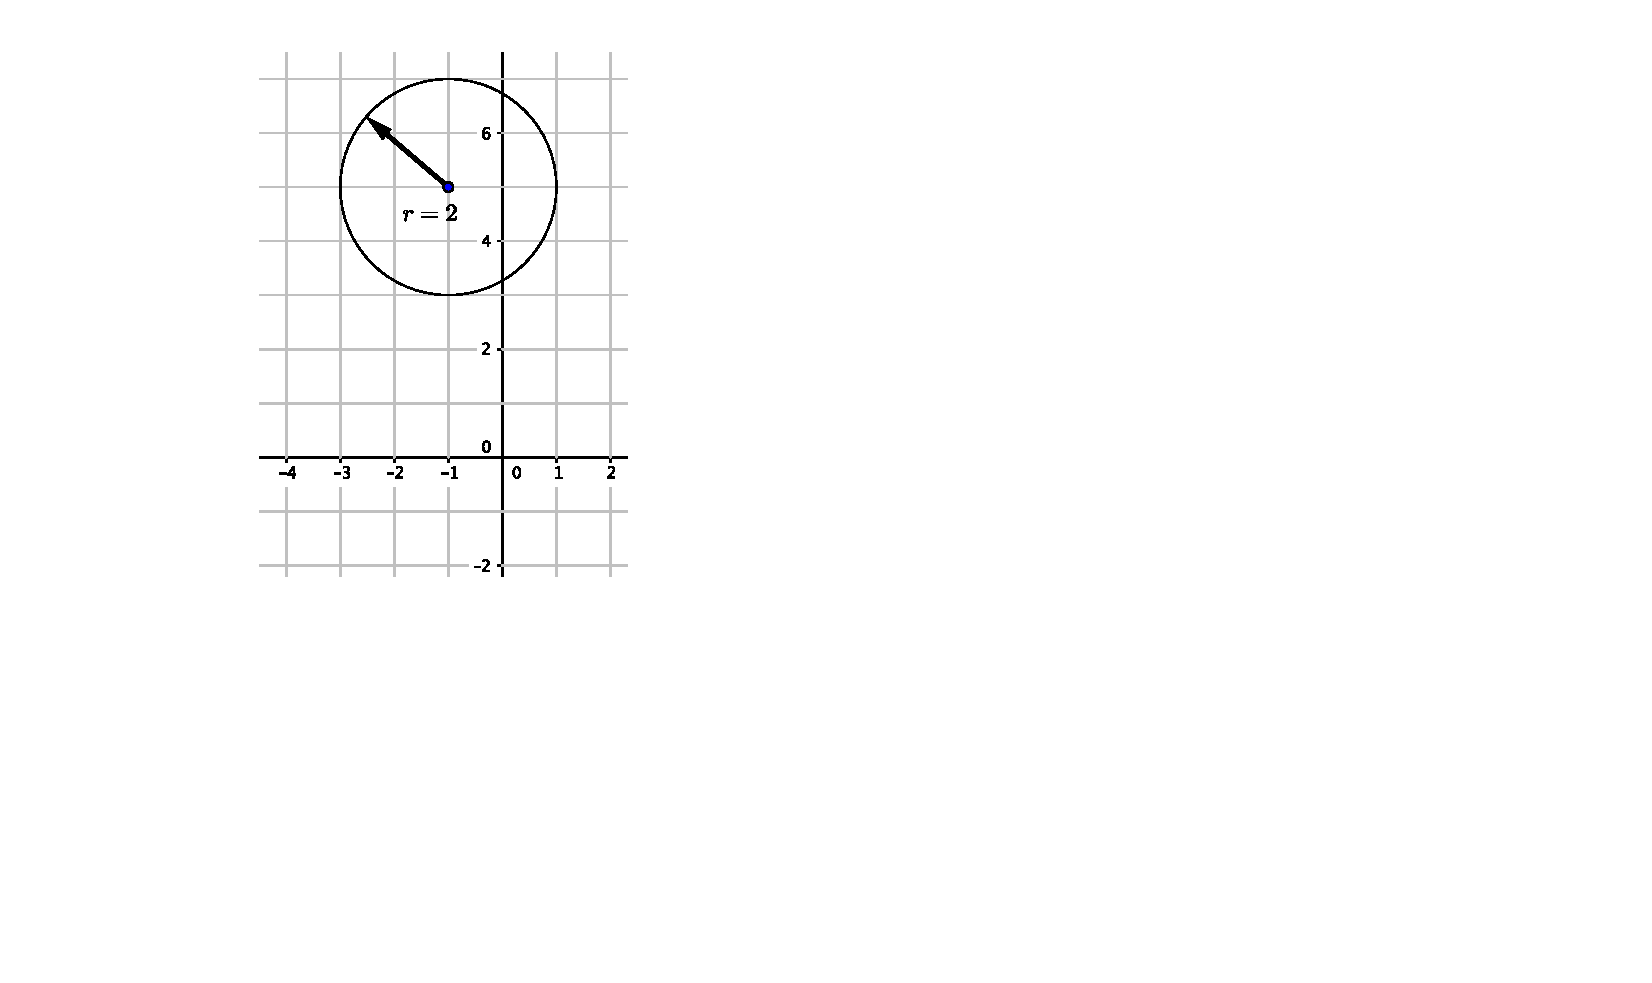
\includegraphics[height=2.5in]{MAT100_Number21c.pdf}}
{\begin{tabular}{lllll}
 &&&&\\ Correct form of the equations&&$(x-h)^2+(y-k)^2=r^2$&&Add 2 points\\
Correct center of the circle&&$(-1,5)$&&Add 2 points\\
Correct radius of the equation&&$r=2$&&Add 2 points\\ &&&&\\ \end{tabular}}


\newproblem{21.5d} 
{Find the equation of the circle graphed below.

\noindent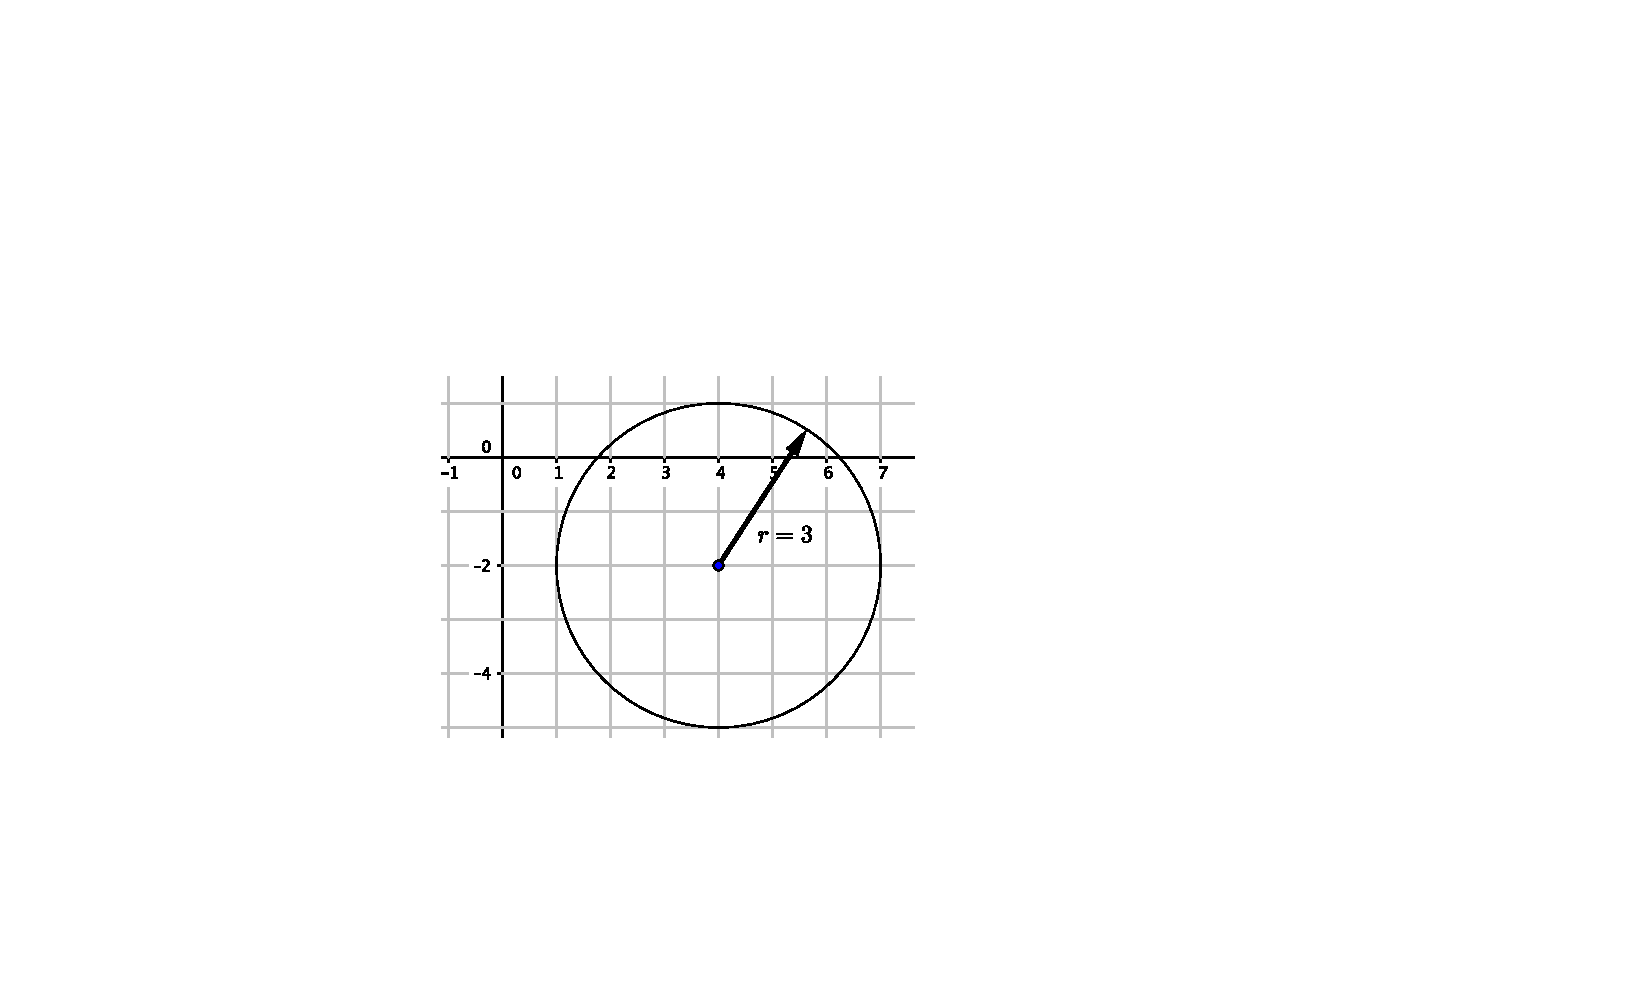
\includegraphics[height=2.5in]{MAT100_Number21d.pdf}}
{\begin{tabular}{lllll}
 &&&&\\ Correct form of the equations&&$(x-h)^2+(y-k)^2=r^2$&&Add 2 points\\
Correct center of the circle&&$(4,-2)$&&Add 2 points\\
Correct radius of the equation&&$r=3$&&Add 2 points\\ &&&&\\ \end{tabular}}
